% !TeX root = ../note.tex
\section{Обзор предметной области}\label{sec:analysis}

Конечный успех программного проекта во многом определяется до начала конструирования: на этапе подготовки, которая проводится с учетом всех особенностей проекта.
\par
Первое предварительное условие, которое нужно выполнить перед конструированием, – ясное формулирование проблемы, которую система должна решать. Общая цель подготовки — снижение риска: адекватное планирование позволяет исключить главные аспекты риска на самых ранних стадиях работы, чтобы основную часть проекта можно было выполнить максимально эффективно.
\par
Главный факторы риска в создании ПО — неудачная выработка требований. Требования подробно описывают, что должна делать программная система. Внимание к требованиям помогает свести к минимуму изменения системы после начала разработки~\cite{code_complete}.
\par
Перед формулированием требований необходимо изучить ряд вопросов, которые напрямую влияют на все дальнейшие этапы разработки. В частности, необходимо рассмотреть вопросы выбора платформ, архитектуры. По результатам анализа можно будет составить техническое задание к проектируемому программному средству, которое станет основой для составления функциональных требований.
\par
Данный раздел содержит обзор предметной области по теме дипломного проекта, аналоги создаваемого программного продукта, анализ их достоинств и недостатков. На основе проведенного анализа и с учетом требований формулируются требования к проектируемому программному средству.

% !TeX root = ../note.tex
\subsection{Постановка задачи}\label{sec:analysis:task}

Цель настоящего дипломного проекта состоит в разработке программного средства для обработки данных валютной биржи. Перед формированием полноценных требований определим некоторые общие характеристики, которые будут требоваться от конечной реализации (данные характеристики будут уточнены поздней):
\begin{itemize}
    \item ПС должно быть равным или превосходить по скорости рассмотренные далее аналогичные проекты;
    \item архитектура ПС должна соответствовать принципам построения СОА;
    \item отказоустойчивость конечной системы, при которой каждый сервис гарантирует собственную отказоустойчивость.
    \item ПС должно служить в качестве high-load системы;
    \item API ПС должен быть совместимым с современными технологиями back-end программирования.
\end{itemize}


% !TeX root = ../note.tex
\subsection{Обзор существующих аналогов}\label{sec:analysis:analogues}

В данном разделе рассмотрим существующие аналоги, а именно системы, обладающие механизмами для создания ордеров, совершения сделок и другим соответствующим функционалом.

% \subsubsection{} Jira\label{sec:analysis:analogue_1}
\bigskip
\textbf{Jira}

Jira~\cite{analogue_1} позиционируется как коммерческая система отслеживания ошибок, разработана компанией Atlassian. Основной элемент учёта в системе — задача, которая содержит название проекта, тему, тип, приоритет, компоненты и содержание. Она может быть расширена дополнительными полями, различными приложениями (например — фотографиями, скриншотами и т.д.) или комментариями. Среди возможностей данной программы:
\begin{itemize}
    \item Kanban-доска — помогают команде обеспечить прозрачность работы над проектом, оптимизировать рабочий процесс, распределить задачи из списка нерешённых задач. Пример такой доски представлен на рисунке~\ref{fig:analysis:analogue_1:picture};
    \item Scrum-доска — позволяет управлять сложным проектом, объединить команды из разных направлений разработки продукта для достижений одной цели;
    \item отчёты формируются при помощи виджетов на панели дашбордов и могут содержать информацию о проекте в целом или об отдельных его элементах. Отчёты визуализируются в графики и диаграммы.
\end{itemize}

\begin{figure}[ht]
    \centering
	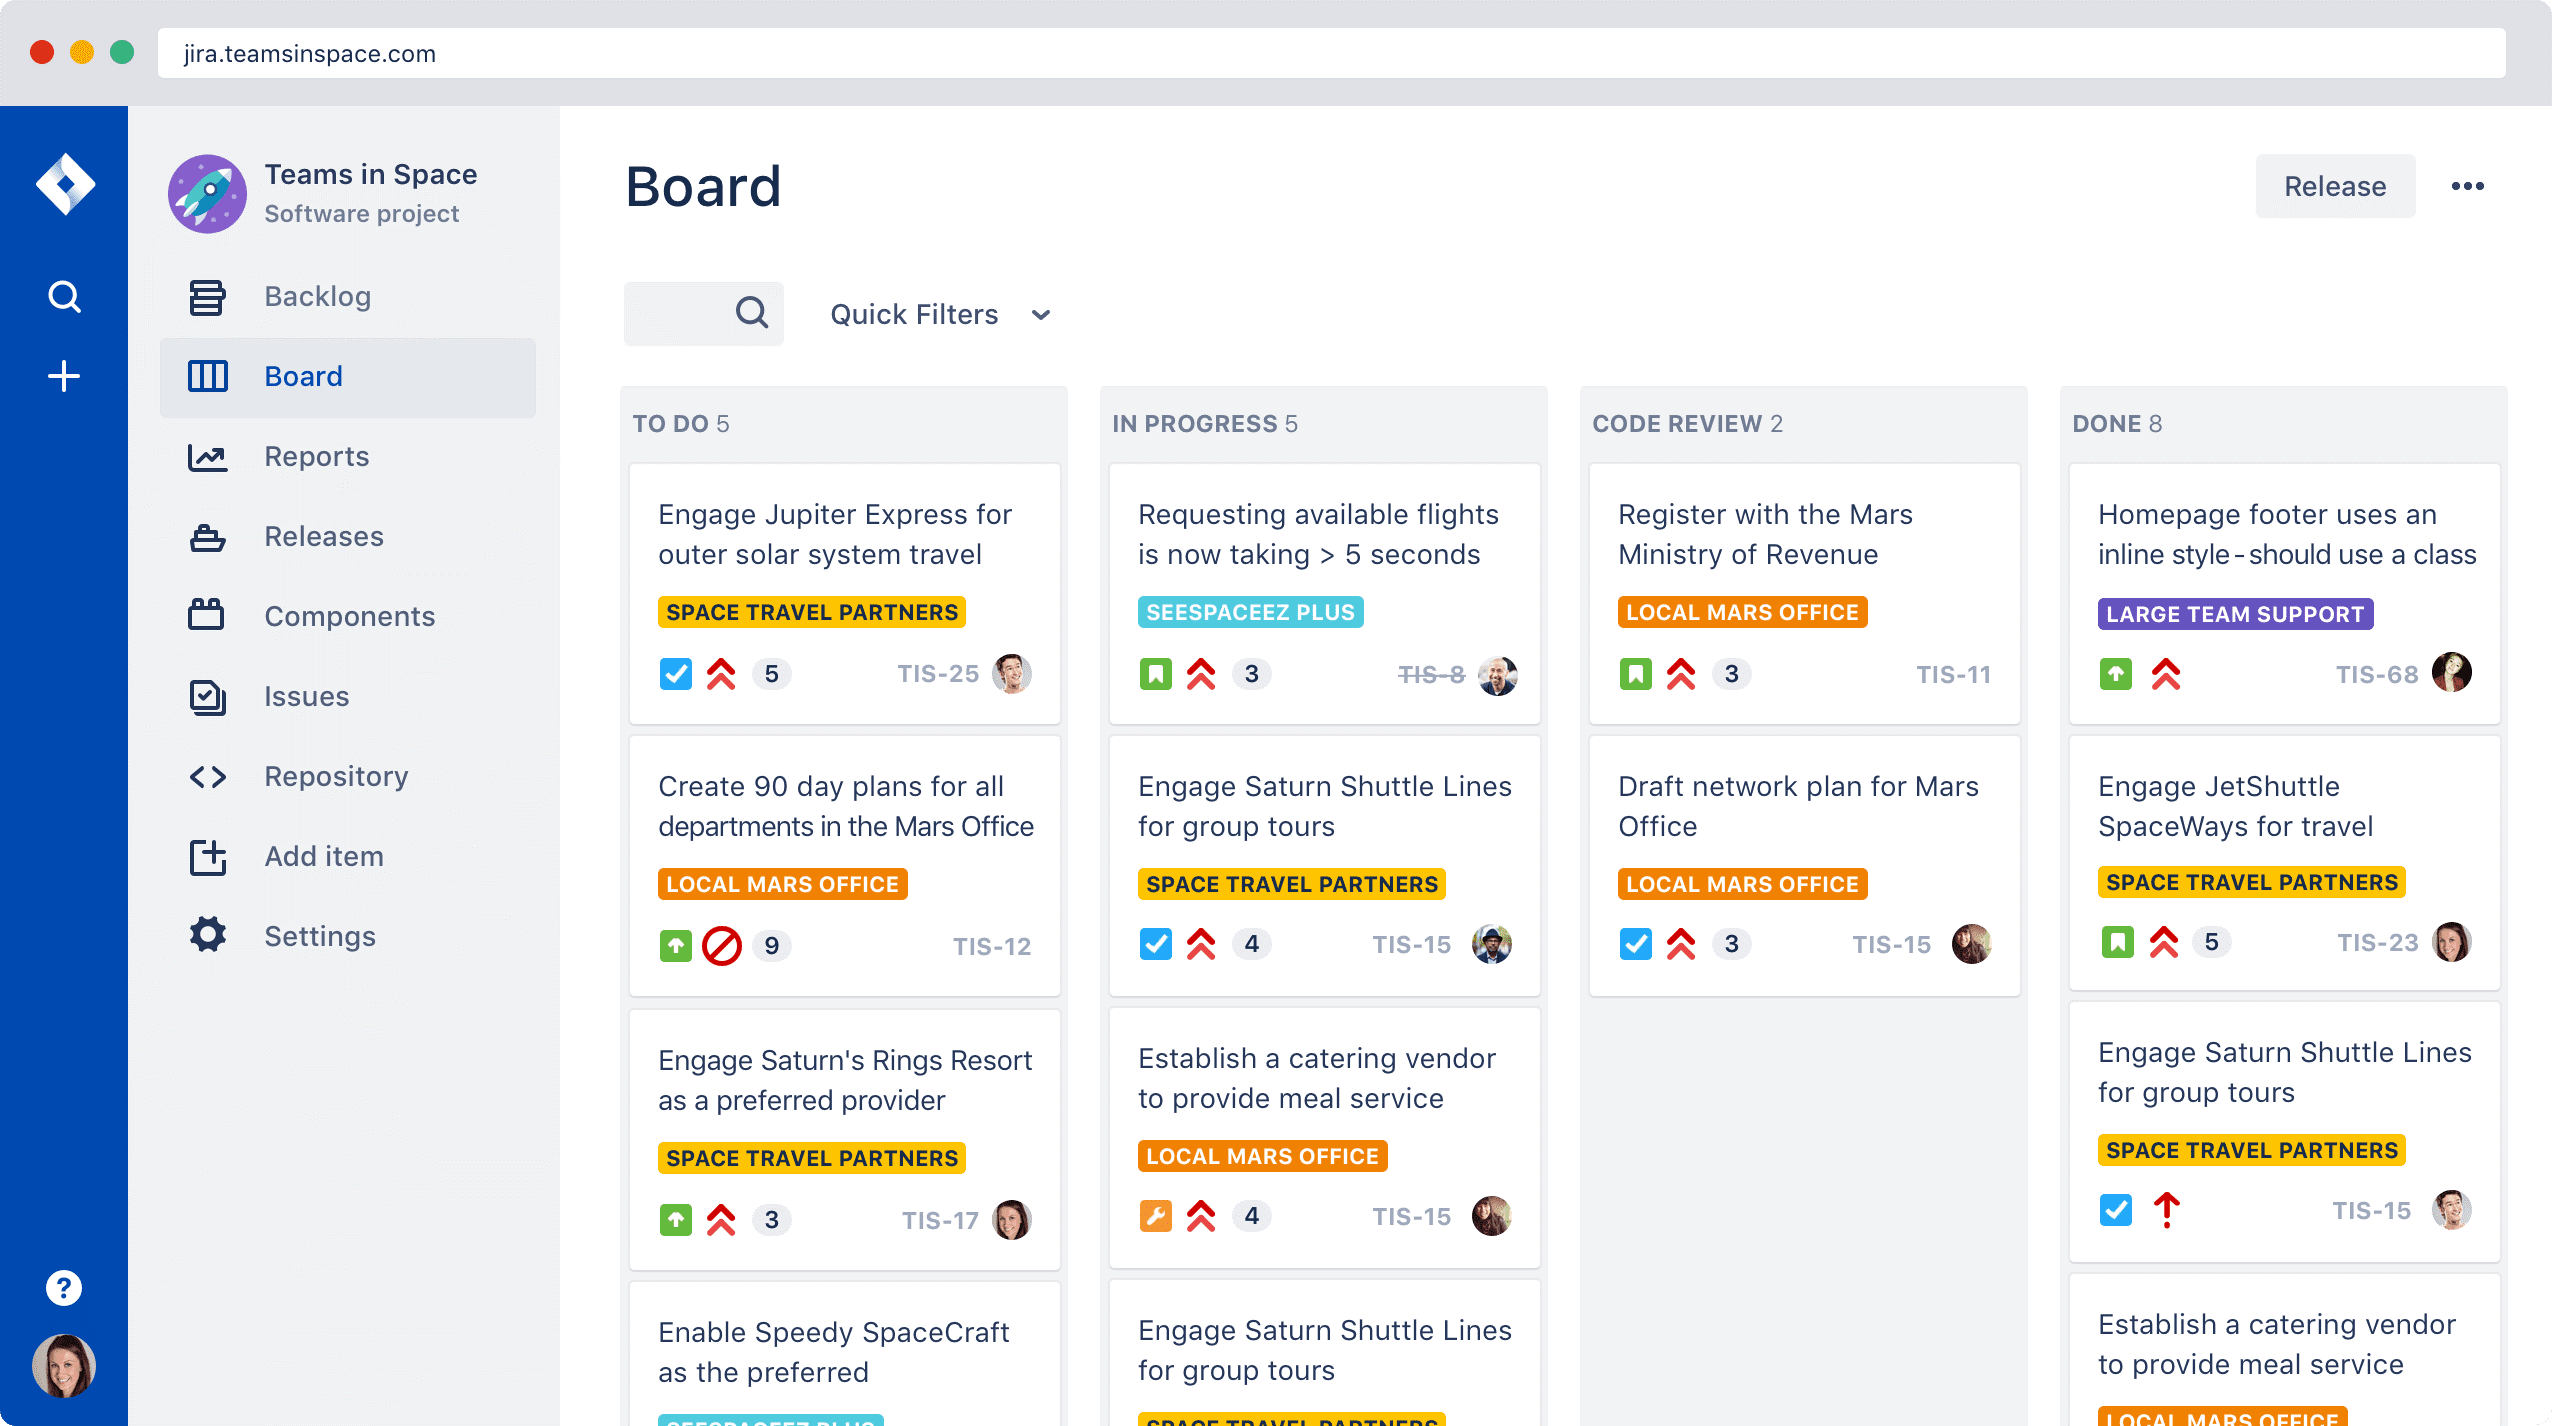
\includegraphics[width=\textwidth]{analogue_1.png}
	\caption{Пример Kanban-доски в системе Jira}\label{fig:analysis:analogue_1:picture}
\end{figure}

Из плюсов данного проекта можно отметить:
\begin{itemize}
    \item огромное количество функционала для эффективной работы над проектами;
    \item поддержка интеграций с множеством инструментов для разработки и других сервисов;
    \item широкая кастомизация, которая позволяет с лёгкостью адаптироваться под нужды конкретных заказчиков.
\end{itemize}

К минусам данного ПО можно отнести:
\begin{itemize}
    \item высокая цена с привязкой к количеству пользователей;
    \item сложный интерфейс;
    \item отсутствие по умолчанию функционала для работы с персоналом.
\end{itemize}

\bigskip
\textbf{YouTrack}

YouTrack — коммерческая система отслеживания ошибок, разработана компанией JetBrains~\cite{analogue_2}. Система поддерживает поисковые запросы, автодополнение, создание пользовательских рабочих процессов. Стандартные интеграции YouTrack включают импорт из Jira, интеграции с электронными почтовыми ящиками, c Zendesk, единую рабочую среду с Upsource и TeamCity, а также встроенную интеграцию с системами контроля версий GitHub, BitBucket и GitLab.

\begin{figure}[ht]
    \centering
	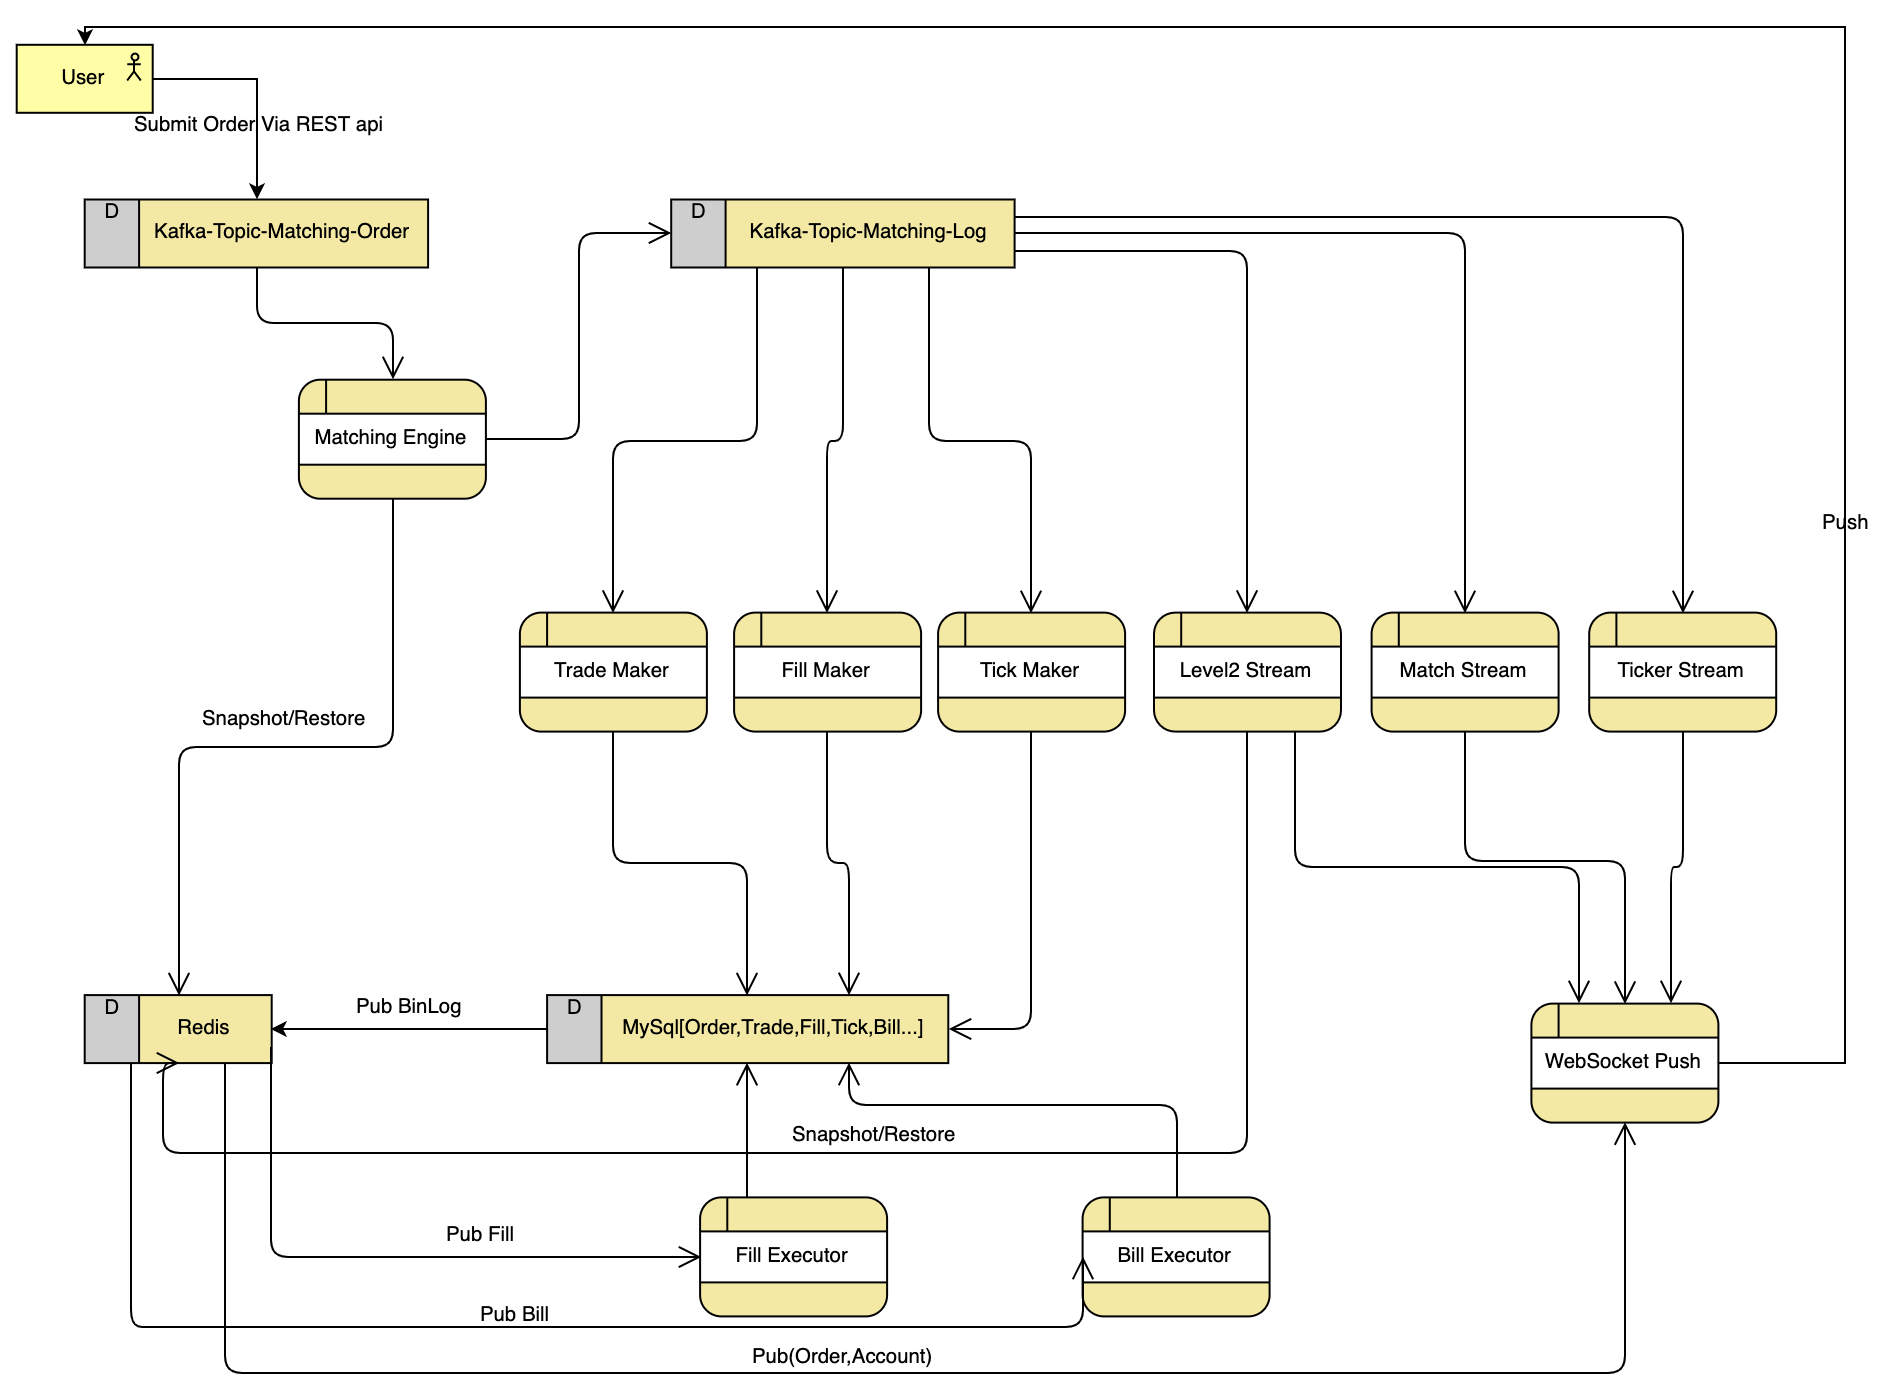
\includegraphics[width=\textwidth]{analogue_2.png}
	\caption{Пример доски в системе YouTrack}\label{fig:analysis:analogue_2:picture}
\end{figure}

В данном проекте можно отметить как плюсы следующее:
\begin{itemize}
    \item Scrum и Kanban доски для визуализации процесса разработки. Пример доски представлен на рисунке~\ref{fig:analysis:analogue_2:picture};
    \item интеллектуальный поиск при помощи поисковых запросов с подсказками и подсветкой ошибок;
    \item возможность применения команд для быстрого изменения нескольких задач сразу;
    \item Экспорт в CSV;
    \item поддержка интеграции с IDE от JetBrains: IntelliJ IDEA, PhpStorm, WebStorm, PyCharm, RubyMine, CLion, Rider, GoLand и AppCode.
\end{itemize}

К минусам данного ПО можно отнести:
\begin{itemize}
    \item высокая цена;
    \item небольшие проблемы с производительностью;
    \item отсутствие функционала для работы с персоналом.
\end{itemize}

\bigskip
\textbf{Trello}

Trello — облачная программа для управления проектами небольших групп, разработанная Fog Creek Software~\cite{analogue_3}. В Trello основной упор сделан на пачки карточек. Каждая пачка показывает состояние любого проекта. Карточки имеют множество возможностей. Они предназначены для обсуждений, голосований, загрузки файлов и данных. Есть возможность задавать дедлайны, назначать текстовые и цветовые метки.

\begin{figure}[ht]
    \centering
	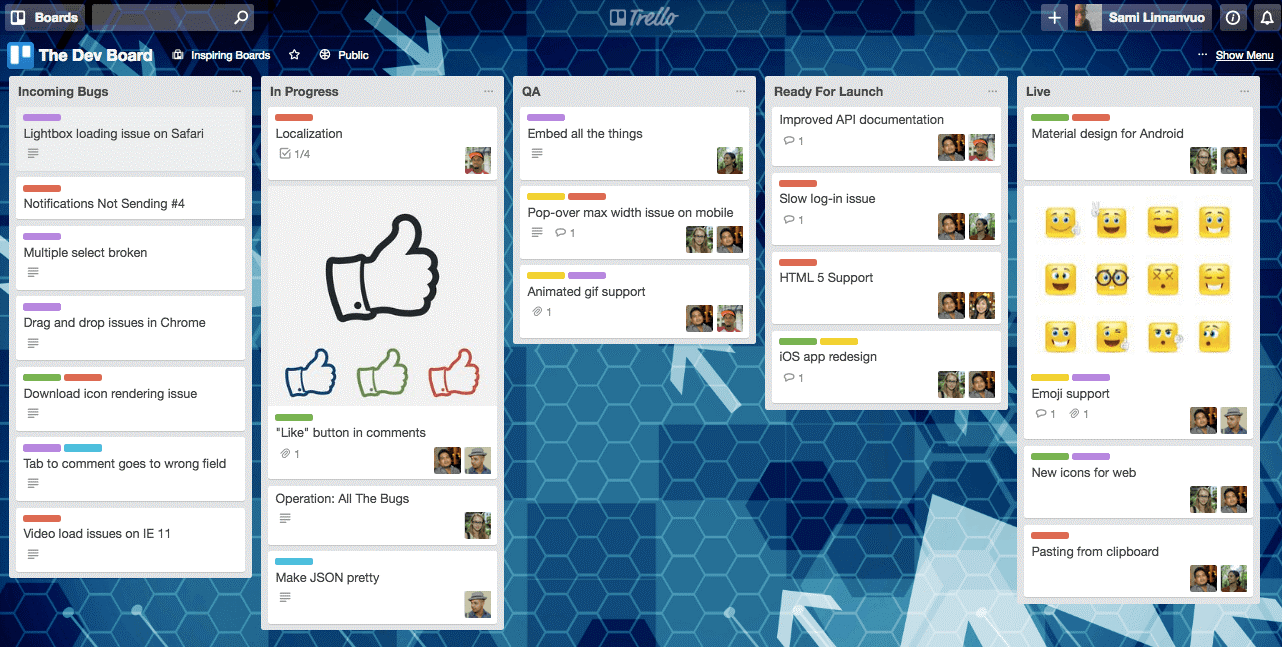
\includegraphics[width=\textwidth]{analogue_3.png}
	\caption{Пример доски в системе Trello}\label{fig:analysis:analogue_3:picture}
\end{figure}

Из сильных сторон проекта можно выделить:
\begin{itemize}
    \item Kanban-доски, которые помогают команде обеспечить прозрачность работы над проектом, оптимизировать рабочий процесс, распределить задачи из списка нерешённых задач. Пример такой доски представлен на рисунке~\ref{fig:analysis:analogue_3:picture};
    \item удобная и широко настраиваемая система уведомлений;
    \item наличие мобильной версии;
    \item низкая цена.
\end{itemize}

К минусам данного ПО можно отнести:
\begin{itemize}
    \item малое количество штатных средств для форматирования текста на карточках;
    \item малая интеграция со сторонними сервисами;
    \item отсутствие функционала для работы с персоналом.
\end{itemize}

\bigskip
\textbf{Azure DevOps Server}

Azure DevOps Server – продукт корпорации Microsoft, представляющий собой комплексное решение~\cite{analogue_4}, объединяющее в себе систему управления версиями, сбор данных, построение отчётов, отслеживание статусов и изменений по проекту и предназначенное для совместной работы над проектами по разработке программного обеспечения.

Из сильных сторон проекта можно отметить:
\begin{itemize}
    \item Kanban-доски, которые помогают команде обеспечить прозрачность работы над проектом, оптимизировать рабочий процесс, а также распределить задачи из списка нерешённых задач;
    \item Scrum-доска, которая позволяет управлять сложным проектом, объединить команды из разных направлений разработки продукта для достижений одной цели;
    \item возможность привязки программного кода к задачам при помощи собственного репозитория управления исходным кодом;
    \item автоматическое создание SharePoint-сайта для проекта, который может использоваться для отслеживания прогресса проекта, наблюдения за рабочими элементами и документами, представленными в библиотеке проекта.
\end{itemize}

К минусам данного ПО можно отнести:
\begin{itemize}
    \item очень высокая цена с привязкой к количеству пользователей;
    \item отсутствие функционала для работы с персоналом.
\end{itemize}

\bigskip
\textbf{Bugzilla}

Bugzilla – свободная система отслеживания ошибок с веб-интерфейсом. Системой Bugzilla пользуются, в числе прочих, Mozilla Foundation, WebKit, Linux kernel, FreeBSD, KDE, Apache, Red Hat, Eclipse и LibreOffice.

Из сильных сторон проекта можно отметить:
\begin{itemize}
    \item расширенный поиск;
    \item уведомления по электронной почте;
    \item списки ошибок в различных форматах;
    \item регулярные отчёты по электронной почте;
    \item отчёты и графики;
    \item автообнаружение дубликатов багов;
    \item изменение задач по электронной почте;
    \item отслеживание времени;
    \item вложения и комментарии.
\end{itemize}

К минусам данного ПО можно отнести:
\begin{itemize}
    \item сложность установки;
    \item зависимость от модулей Perl;
    \item сложность администрирования;
    \item отсутствие функционала для работы с персоналом.
\end{itemize}


% !TeX root = ../note.tex
\subsection{Требования к проектируемому программному средству}\label{sec:analysis:specification}

По результатам изучения предметной области, анализа литературных источников и обзора существующих систем-аналогов сформулируем список основных сервисов и модулей, необходимых для проектирования и реализации программного средства.

\bigskip
\textbf{Функциональные требования}

В данном дипломном проекте должна использоваться сервис-ориенти\-рованная архитектура, так как она позволяет легко развивать приложение в соответствии с нуждами пользователей. Именно поэтому необходимо выделить и описать сервисы и модули, которые будут частями конечного продукта. Должны быть реализованы следующие сервисы:
\begin{itemize}
    \item employee development service — сервис, который обрабатывает профессиональную информацию пользователей, хранит и обновляет задачи и цели развития;
    \item project management service — сервис, который хранит и обрабатывает информацию о проектах;
    \item file service — сервис, который используется для загрузки и получения пользовательских файлов;
    \item notification service — сервис, который обрабатывает события об отправке уведомлений пользователям;
    \item authority service — сервис, который отвечает за хранение идентификационных данных пользователей и их аутентификацию и авторизацию.
\end{itemize}

Все сервисы должны включать в себя такие модули, как:
\begin{itemize}
    \item логирование — для отслеживания действий, происходящих в сервисе; поиска и отладки возможных ошибок;
    \item работа с БД — для хранения и обновления данных сервисов;
    \item конфигурация — модуль должен содержать опции, которые позволяют настраивать сервисы при запуске;
    \item восстановление данных — модуль должен восстанавливать данные в случае перезапуска сервиса;
    \item сериализация данных — для обмена данными между сервисами необходимо определить единый способ сериализации/десериализации данных.
\end{itemize}

Для сервисов employee development и project management также актуальны следующие модули:
\begin{itemize}
    \item UI — пользователь должен иметь возможность быстро и удобно получить актуальную информацию;
    \item события для межсервисного взаимодействия — для своевременного уведомления пользователей об изменениях.
\end{itemize}

\bigskip
\textbf{Нефункциональные требования}

Из нефункциональных требований можно выделить следующие:
\begin{itemize}
    \item написание ПС на одном из быстрых языков программирования, таких как С/С++/\csharp или Rust;
    \item использование СУБД, которые способны эффективно обрабатывать данные, которые хранят сервисы разрабатываемого ПО;
    \item использование надёжного протокола авторизации.
\end{itemize}

